%!TeX program = xelatex
%!TeX builder = latexmk
\documentclass{mcmthesis}
\mcmsetup{tcn = 88277, problem = B}
\usepackage{blindtext}      % 提供 \blindtext 命令,演示用
\usepackage{subfigure}
\usepackage{caption}

\title{The Title}
\author{Team 88277}
\date{\today}

\begin{document}
% 摘要
\begin{abstract}
abstract content blablabla \\
next line
% 用 \\ 换行
% 关键字
\begin{keywords}
keyword1; keyword2
\end{keywords}

\end{abstract}

\maketitle                  % 生成前面的摘要页和标题页
\tableofcontents
% 介绍 Introduction
\section{Introduction}
instroduction content
% section
\section{Establishing Energy profile}
Our aim is to use the Energy profile to represent the total annual consumption of various energy
sources and their structure. According to the official website of the data introduction,
we divide energy into five categories which are Coal, Natural Gas, Petroleum, Renewable Energy and Nuclear electric power.
This energy profile includes the annual consumption of five energy sources and describes their changes from 1960 to 2009.
In addition, we use the annual energy consumption of the five major energy sources
in different industries to reflect changes in the use of different types of energy in different industries
\subsection{Data analysis and preparation}

\subsubsection{Energy classification}
Energy sources have been classified into five main kinds. Each class has some variables which listed in the memo page.
\begin{itemize}
    \item Coal\\
    Includes coal($CL$) and coal coke($CC$). Recorded as $coal$ . Then $coal = \{CL, CC\}$
    \item Natural Gas\\
    Includes natural gas ($NN$). Recorded as $ng$ . Then $ng = \{NN\}$
    \item Petroleum\\
    Includes aviation gasoline($AB$), crude oil($CO$), fossile fuels ($ff$), jet fuel($JF$) etc.
    Recorded as $petro$. Then $petro = \{AB, AR, AV, CO, DF, FF, FN, ... \}$. More variables are listed in the memo page.
    \item Renewable Energy\\
    Includes fuel ethanol($EN$), geothermal energy($GE$), solar energy($GO$), wind($WY$) and wood($WD$) etc.
    Recorded as $re$ . Then $re = \{BM, EN, EM, ES, GE, GO, ... \}$
    \item Nuclear electric power\\
    Includes nuclear electric power($NU$). Recorded as $nu$ . Then $nu = \{NU\}$
\end{itemize}
\subsubsection{Four kinds of industries}
\begin{itemize}
  \item Residential sector\\
  An energy-consuming sector that consists of living quarters for private households.\\
  We choose to use $RCB$ (residential energy consumption, data in British thermal units (Btu)) to measure its energy consumption.
  \item Commercial sector\\
  An energy-consuming sector that consists of service-providing facilities and equipment of: businesses; federal,
  state, and local governments; and other private and public organizations. The commercial sector includes
  institutional living quarters. It also includes sewage treatment facilities.\\
  We choose to use $CCB$ (commercial energy consumption, data in British thermal units (Btu)) to measure its energy consumption.
  \item Industrial sector\\
  An energy-consuming sector that consists of all facilities and equipment used for producing, processing, or assembling goods.\\
  We chose to use $ICB$ (Industrial energy consumption, data in British thermal units (Btu)) to measure its energy consumption.
  \item Transportation sector\\
  An energy-consuming sector that consists of all vehicles whose primary purpose is transporting people and/or
  goods from one physical location to another.\\
  We chose to use $TCB$ (Transportation energy consumption, data in British thermal units (Btu)) to measure its energy consumption.
\end{itemize}
\subsubsection{The calculation process}
\begin{itemize}
  \item Calculation of the total consumption of five kinds of energy sources
  Filter the given variables. What we need is the total annual consumption of each kind energy sources.
  For example, the total consumption of coal($coalTCB$) is $CLTCB + CCTCB$. \\
  The more general way to represent the total consumption of each kind energy sources is\\
  $$coalTCB = \sum_{i=0}^{n} var_iTCB  \ \ \ var_i \in coal, n = |coal| \\$$
  $$ngTCB = \sum_{i=0}^{n} var_iTCB  \ \ \ var_i \in ng, n = |ng| \\$$
  $$petroTCB = \sum_{i=0}^{n} var_iTCB  \ \ \ var_i \in petro, n = |petro| \\$$
  $$reTCB = \sum_{i=0}^{n} var_iTCB  \ \ \ var_i \in re, n = |re|$$
  $$nuTCB = \sum_{i=0}^{n} var_iTCB  \ \ \ var_i \in nu, n = |nu|$$
  \item Calculate the consumption of five kinds of energy sources in four sectors separately
  From the data, we choose the energy consumption of all energy sources in each sector and then add up according to the sector.
  For example, $coalRCB$ (consumption of coal in the residential sector) is: $CLRCB + CCRCB$ .
  As well, use symbols to represent this is
  $$coalACB = \sum_{i=0}^{n} var_iACB  \ \ \ var_i \in coal, n = |coal| \\$$
  $$coalCCB = \sum_{i=0}^{n} var_iCCB  \ \ \ var_i \in coal, n = |coal| \\$$
  $$coalICB = \sum_{i=0}^{n} var_iICB  \ \ \ var_i \in coal, n = |coal| \\$$
  $$coalRCB = \sum_{i=0}^{n} var_iRCB  \ \ \ var_i \in coal, n = |coal| \\$$
  $$ngACB = \sum_{i=0}^{n} var_iACB  \ \ \ var_i \in ng, n = |ng| \\$$
  $$ngCCB = \sum_{i=0}^{n} var_iCCB  \ \ \ var_i \in ng, n = |ng| \\$$
  $$ngICB = \sum_{i=0}^{n} var_iICB  \ \ \ var_i \in ng, n = |ng| \\$$
  $$ngRCB = \sum_{i=0}^{n} var_iRCB  \ \ \ var_i \in ng, n = |ng| \\$$
  And the rest three kinds of energy sources ($petro, re\ and\ nu$) have similar formula.
\end{itemize}
\subsubsection{Formula for energy profile}
To get the final formula, we have one step to do. Use every kinds of annual consumption to divide it own fields of total annual consumption.
Such as, record the total energy annual consumption is $TETCB$, and the result of using $coalTCB$ to devide $TETCB$ is noted as $coalVT$.
$$coalVT = \frac{coalTCB}{TETCB}$$
And use $coalVA$ to record $coalACB$ to devide $TEACB$.
$$coalVA = \frac{coalACB}{TEACB}$$
More variables have been listed in the memo page.\\
The final representation of the formula is
$$
  EP =
  \begin{pmatrix}
  coalVT & coalVA & coalVC & coalVI & coalVR  \\
  ngVT & ngVA & ngVC & ngVI & ngVR \\
  petroVT & petroVA & petroVC & petroVI & petroVR \\
  reVT & reVA & reVC & reVI & reVR \\
  nuVT & 0 & 0 & 0 & 0\\
  \end{pmatrix}
$$

* Note that Nuclear electric power doesn't have variables to represent the annual consumption in different sectors.
But it is still an important energy sources, so we keep it.

\subsection{California' energy profile}
Stretching two-thirds of the way up the West Coast, California is the nation's third-largest state,and also California is the most populated state in the nation, and, with the largest economy, its total energy demand is second only to Texas. California's extensive efforts to increase energy efficiency, along with the implementation of alternative technologies, has restrained growth in energy demand. California is also rich in energy resources. The state has an abundant supply of crude oil and is a top producer of conventional hydroelectric power. California also leads the nation in electricity generation from solar, geothermal, and biomass resources. Transportation dominates California's energy consumption profile. More motor vehicles are registered in California than in any other state, and commute times in California are among the longest in the country. The state also accounts for one-fifth of the nation's jet fuel consumption.

\subsubsection{Petroleum}
  For California, oil is its primary source of energy, with oil accounting for more than $60\%$ of total energy consumption in the past 50 years. However, it can be seen that the share of oil in total consumption after constant technological innovation Showing a weak downward trend. In particular, in the industrial sector, the proportion of oil used in the past few years has dropped in volatility and has been shown to complement each other with natural gas. With the growth in the use of natural gas, oil may be gradually replaced. However, in the transportation sector, the share of oil used is close to $100\%$ and there is no downward trend. In the commercial and residential sectors, the proportion of oil used has risen to some extent, reaching around $40\%$ and $50\%$ in 2009. It shows that California is very dependent on oil. Although the overall trend is declining, it can not leave the oil in the short term.
\subsubsection{Natural gas}
  California accounts for less than $1\%$ of total U.S. natural gas reserves and production. After the 1970s, California's natural gas production experienced a gradual and complete decline over the past 30 years. From $30\%$ in the 1960s and now up and down at $20\%$. The demand for natural gas in California is not so strong, and from the data analysis, it has been relatively stable at about $20\%$ in recent years. The use of natural gas in the dwelling sector has dropped continuously from $80\%$ to $45\%$ in 50 years. The same is true of the commercial sector, which started to decline continuously after rising to $70\%$ in the 1970s and reached $25\%$ in 2009. Contrary to the previous one, the industrial sector seems to consider natural gas as a substitute for petroleum. After a decline in the 1970s, it rose from fluctuations in the mid-1980s to a $47\%$ share and is still on the rise.
\subsubsection{Renewable energy}
  California is among the top states in the nation in electricity generation from renewable resources and leads the nation in generation from solar, geothermal, and biomass energy. California is also the nation's third-largest producer of electricity from conventional hydroelectric power and the fifth-largest producer from wind energy. With the development of science and technology, the ratio of renewable energy sources shows a steady and steady rise in total energy consumption. This is evident in the residential and commercial sectors and has been rising for 50 years. In the residential sector, the share rose from $8\%$ to $17\%$ and in commerce from $12\%$ to $23\%$, but the charts in recent years show that the rate of increase is declining steadily. In industry, however, the share of renewable energy in the last 50 years was the highest since the oil crisis, and the share of renewable energy declined after the 1970s, recovering slightly from 2000 to 2009.
\subsubsection{Coal}
  California does not have any coal reserves or production and has phased out almost all use of coal for electricity generation. As you can see from the table, California's demand for coal is extremely low, even lower than the demand for renewable energy in 2000-2009. No matter in the commercial, transportation, residential or industrial sectors, there is an extremely low proportion of those coming out to zero and there is no continuing upward trend.
  \begin{figure}[htbp]
  \centering
  \begin{minipage}[t]{0.48\textwidth}
  \centering
  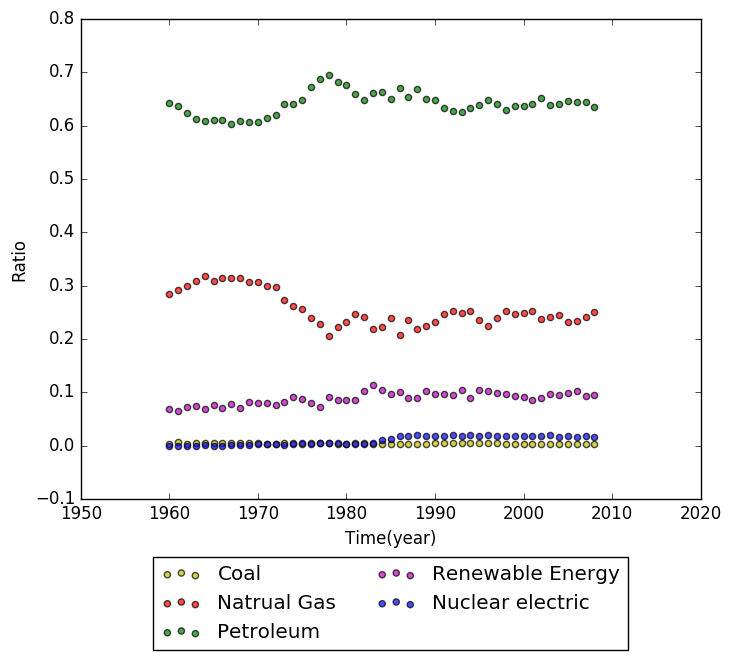
\includegraphics[width=6cm]{energyprofile_ca.png}
  \captionsetup{font={small}}
  \caption{Energy consumption, California}
  \end{minipage}
  \begin{minipage}[t]{0.48\textwidth}
  \centering
  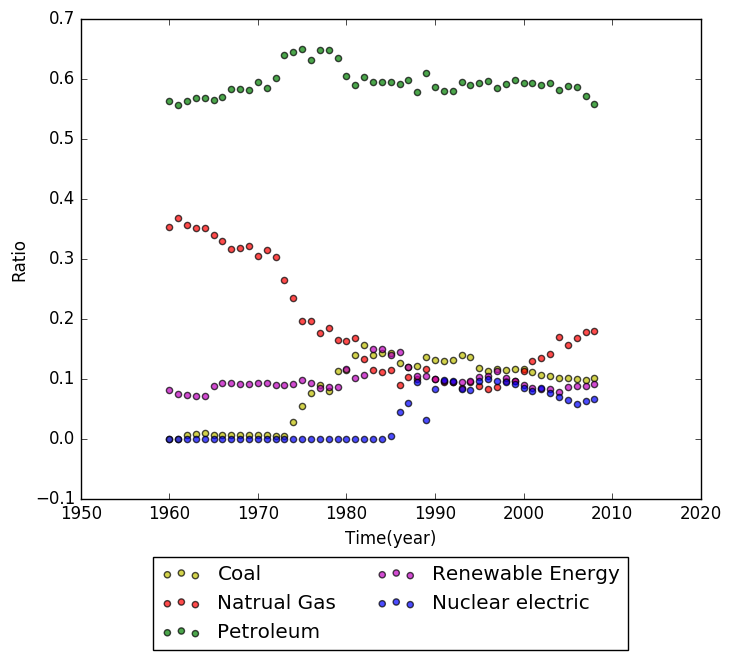
\includegraphics[width=6cm]{energyprofile_az.png}
  \captionsetup{font={small}}
  \caption{Energy consumption, Arizona}
  \end{minipage}
  \end{figure}
\subsection{Arizona' energy profile}
Arizona is known for its iconic vistas from the Grand Canyon in the north to the Saguaro deserts in the south. The state has few fossil fuel resources, but it does have abundant solar and geothermal energy potential. Elevations in Arizona vary from peaks more than 12,000 feet high in the north to nearly sea level in the lower deserts to the southwest. And abundant sunshine gives the entire state some of the nation’s greatest solar power potential. Because the main economic activity in Arizona is not energy-intensive, the country's per capita energy consumption is the lowest in the country. The transportation sector is the largest consumer of terminal energy in Arizona, followed by the residential market. The main energy source in Arizona is oil.
\subsection{Petroleum}
  Arizona does not have any refinery. Gasoline and other petroleum products are supplied by pipelines in Southern California and Texas.
  The transportation sector, which is the most dependent on oil, has risen to about 2005 from the 1960s, rising almost from $82\%$ to $95\%$.
  Since 2005, the share of renewables and natural gas has slightly declined. According to calculations, nearly ten barrels of oil will be
  used for the transport sector and the rest will be basically used in the industrial sector. The use of oil in the industrial sector
  as a whole is on the rise, rising from $27\%$ to $65\%$ and is still on the rise. In the residential and commercial sectors, the share of
  oil also increased, with the residential sector rising from $16\%$ to $50\%$ and stabilizing, with $30\%$ of the commercial sector turning $52\%$.
  On the whole, Arizona is getting more and more dependent on oil.
\subsection{Natural gas}
  Arizona has no significant gas reserves. The share of natural gas from the 1960s to the 1990s has been declining until it showed an upward
  trend in the late 1990s. In all four key sectors, the use of natural gas, in general, has been declining. In the commercial sector, the
  share of natural gas dropped rapidly from $64\%$ to below $10\%$ from $60\%$ to $20\%$ in the industrial sector and seems to be still on the decline.
  In the industrial sector, from the 1960s to the 1990s, the proportion of natural gas dropped rapidly to below $10\%$ and then to $15\%$.
  And fluctuated around $15\%$ in the 1990s and early twenty-first centuries. In the residential sector, the share of natural gas has been declining,
  from $70\%$ to $15\%$, and the post-term decline has been softer than the previous decline. In the transport sector from
  $22\%$ dropped to about $5\%$, and in 2009 by the rising trend. Natural gas was once one of the main sources of energy in Arizona, but natural
  gas is no longer as important for Arizona as the cost of other energy uses goes down.
\subsection{Renewable Energy}
  Arizona's renewable energy standards require that investors in the power utilities and retail power providers receive more and more electricity
  from renewable sources. Renewable energy has been one of Arizona's major energy sources and its share has been close to $10\%$ between the 1960s
  and the 1980s, with a sharp increase of nearly $15\%$ between 1980 and 1985 , Then retreated. Since 2001, the share of renewable energy has risen
  slowly and has continued to rise. The share of renewable energy in the industry has been rising for 30 consecutive years, up to $20\%$ and
  a slight decrease since the 1990s. However, the proportion of renewable energy in the industry has been on a rising trend since the 21st century.
  Renewable energy in the residential sector has been on the rise, rising from $10\%$ to $25\%$ in 50 years and the energy mix has changed dramatically.
  Commercial and transportation sectors basically do not use renewable energy.
\subsection{Coal}
  Renewable energy Arizona has two coalfields - Black Mesa, the Navajo River and the Northeast Hippo Reservation, Pinedale, south-central Arizona.
  These areas maintain around $1\%$ of the country's coal reserves in producing mines. The only coal mine operating in the state is located in the Black
  Mesa field, one of the 30 largest coal mines in the country. Arizona started to use coal from the 1970s and quickly became a significant $12\%$ energy
  source in the 1980s. It began to slowly decline to $8\%$ (2009) in the early 1990's and remained stable. Industrial coal,
  which grew rapidly from the mid-1970s to the late 1980s, reached $20\%$ at one point and quickly dropped to $8\%$ in the early 1990s and remained stable.
  In addition to the three departments in the industrial sector, coal is basically not used directly.
\subsection{New Mexico's energy profile}
In New Mexico, there are a great deal of forested peaks and valleys of the southern Rocky Mountains, high plateaus of the Great Plains, and many spectacular desert canyons and mesas. Because of the diversity of altitude, the climate of New Mexico is changeable. In the southern desert, it is common for summer temperatures to exceed 100 degrees Fahrenheit. In the northern snow peak, the winter temperature will drop to 50 degrees below zero. New Mexico is with much land but few people. Although it is the fifth-largest state by area, it is the sixth-least densely populated. More than one in four residents live in the city of Albuquerque, and two-thirds of the state has fewer than 10 people per square mile. New Mexico is the nation's 7th largest net energy supply state, rich in fossil fuels, minerals and renewable energy resources. The oil and gas industry, contributes significantly to the state's gross domestic product (GDP), and workers in the sector earn among the highest average weekly pay in the state. New Mexico's energy consumption per dollar of GDP and energy consumption per capita are both above the national average.
\subsubsection{Petroleum}
  New Mexico's crude oil reserves have surpassed $4\%$ of the U.S. It has been the sixth-largest oil producer for a long time, accounting
  for nearly $5\%$ of the country's annual crude output. The Permian Basin in western Texas and southeastern New Mexico are among
  the most productive oil producing areas in the country. The proportion of oil in total energy consumption is as high as more than half.
  From 1960, the proportion of petroleum energy consumption in New Mexico increased year by year, accounting for nearly $60\%$ by the 21st century.
  New Mexico's transportation sector dominates oil consumption. More than $80\%$ of all oil in the state belongs to the sector.
  The industrial sector is far ahead, with only a small amount of oil being used in the residential and commercial sectors.
  Only about $0.1\%$ of New Mexico households use oil products for home heating.
\subsubsection{Natural gas}
  New Mexico, accounting for about $5\%$ of the total natural gas reserves in the United States, is one of the top ten natural gas
  producers in the United States, accounting for about $4\%$ of the country's total natural gas production. Because of the high reserves of
  natural gas, natural gas accounted for as much as $45\%$ of the energy it consumed in the 1970s, comparable to oil.
  However, with the development of oil, coal and renewable energy, the proportion of natural gas in energy consumption has been declining year by year,
  reaching a minimum of $20\%$ in the mid-1980s. From 1990 to 2009, the proportion of natural gas consumption has fluctuated between $20\%$ and $25\%$
   and gradually stabilized.
\subsubsection{Renewable energy}
  New Mexico has a large number of renewable resources, especially wind and solar energy, as well as hydropower, biomass and geothermal energy.
  New Mexico has the sixth-largest geothermal resource in the country. The climate in New Mexico is characterized by ample sunshine.
  And it has developed rapidly in solar technology with the support of national policies. It can be seen that the proportion of energy
  consumption of renewable energy is gradually increasing, approaching $10\%$ by 2009 and there is a trend of continued growth.
  The proportion of energy consumption in the industrial, commercial and residential sectors has increased substantially.
  In particular, the energy consumption of renewable resources in commercial and residential sectors has exceeded $20\%$ by 2009.
\subsubsection{Coal}
  New Mexico contains nearly $3\%$ of the country's estimated recoverable coal reserves. New Mexico has mined coal since the 1850s.
  Therefore, from 1965 to 1985, the proportion of coal's energy consumption gradually increased, reaching a maximum of about $18\%$ in 1985.
  However, with the increase of renewable resources and oil, the proportion of coal's energy consumption has steadily declined.
  Through the analysis of energy consumption in the industrial, transportation, commercial and residential sectors,
  it can be seen that coal accounts for the smallest proportion of energy consumption in all sectors and shows a very small proportion of nearly zero.
  \begin{figure}[htbp]
  \centering
  \begin{minipage}[t]{0.48\textwidth}
  \centering
  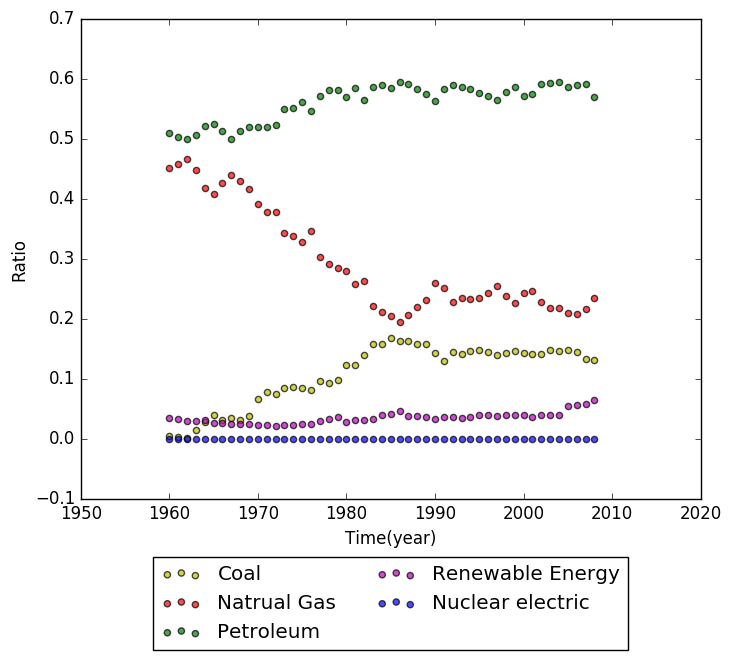
\includegraphics[width=6cm]{energyprofile_nm.png}
  \captionsetup{font={small}}
  \caption{Energy consumption, New Mexico}
  \end{minipage}
  \begin{minipage}[t]{0.48\textwidth}
  \centering
  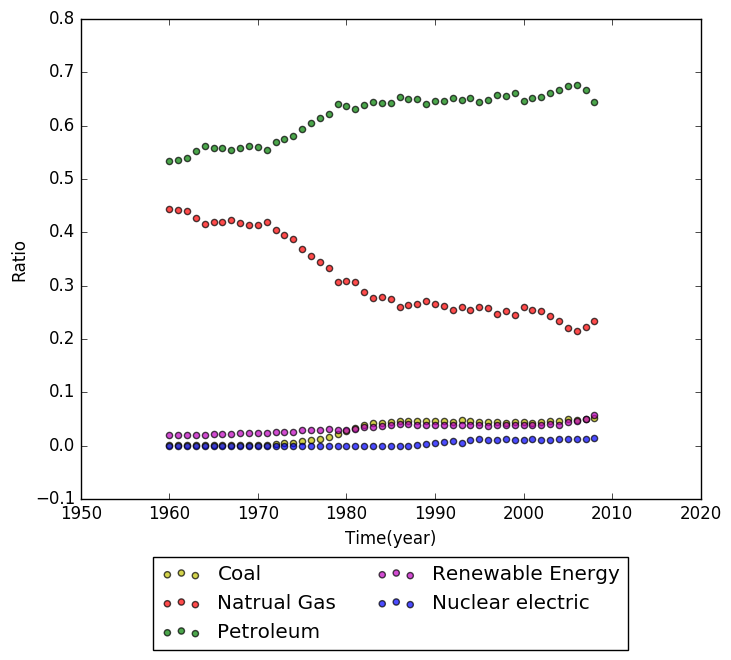
\includegraphics[width=6cm]{energyprofile_tx.png}
  \captionsetup{font={small}}
  \caption{Energy consumption, Texas}
  \end{minipage}
  \end{figure}
\subsection{Texas's energy profile}
Texas, located in the south-central part of the United States, is the second largest in size in the United States. The Texas Almanac classifies the state into four regions: Gulf Coastal Plains, Interior Lowlands, Great Plains, and Basin and Range Province. The Texas climate varies significantly from east to west. Moist air from the Gulf of Mexico sweeps westward across the state, losing moisture as it goes. As a result, the climate ranges from humid and subtropical along the coast, where much of the state's population resides, to semi-arid on the high plains, and arid in the mountainous west. Texas is a large state with a wealth of energy resources. Crude oil and natural gas fields are present across the entire state. Texas also has abundant renewable energy resources and has rapidly developed its wind energy. Besides, Texas is among the leading states in solar energy potential. Among the states, Texas has the second-largest population and the second-largest economy. The state has many energy-intensive industries, including petroleum refining and chemical manufacturing, and the industrial sector accounts for the largest share of state energy use.
\subsubsection{Petroleum}
  Texas is a leader in crude oil reserves and production. More than a third of the U.S. crude oil has been proved reserves.
  More than a quarter of the nation's 100 largest reserves are in Texas, mostly in the Permian Basin in western Texas and south-central Florida.
  More than a third of the country's crude oil is produced in Texas, surpassing any other country and surpassing all federal offshore areas.
  From the discovery of the Spindletop field in 1901 to the subsequent discovery of various oil fields, the proportion of oil in Texas
  in energy consumption gradually increased to $63\%$ in 2009. The proportion of oil consumption is related to that of natural gas.
  The proportion of energy consumption in natural gas is correspondingly increased in the years in which the proportion of petroleum consumption
  is declining, and vice versa. In the industrial, commercial, transport and residential sectors, the proportion of oil in energy consumption is on the rise.
\subsubsection{Natural gas}
  Texas holds one-fourth of the nation's proved natural gas reserves and almost one-third of the 100 largest natural gas fields are located,
  n whole or in part, in the state. Texas also leads the nation in natural gas production, accounting for one-fourth of U.S. However,
  with the increase of oil, coal, renewable resources and nuclear resources, the energy consumption of natural gas has been on the
  whole declining from about $45\%$ in 1960 to about $25\%$ in 2009. In the industrial, commercial and residential sectors,
  by the mid-1970s, the share of natural gas in energy consumption was higher than that in oil, turning around in 1973,
  with the proportion of natural gas being exceeded by oil, and the gap between the two was growing.
\subsubsection{Renewable energy}
  Wind accounts for nearly all of the electricity generated from renewable resources in Texas. The size of the state and
  the high levels of direct solar radiation in West Texas give the state some of the largest solar power potential in the nation.
  The agricultural and forestry sectors can provide Texas with abundant biomass and biofuel resources.
  Despite the large number of non-powered dams in Texas, the potential for further hydroelectric development is limited by lack of precipitation.
  Besides, Texas has a unique untapped geothermal resource: its large network of crude oil and natural gas wells. 
  Renewable resources in Texas, the proportion of energy consumption increased year by year.
  In particular, the proportion of energy in the commercial and residential sectors has been as high as $25\%$ to $30\%$.
\subsubsection{Coal}
  Texas found large lignite coal mines in the narrow belt of Texas Gulf Coast, as well as bituminous coal deposits in north-central
  and southwestern Texas. Overall, the state estimates recoverable reserves of more than 9 billion tons.
  Texas is the seventh largest coal producer and the nation's largest lignite producer. Texas is the largest coal-consuming nation
  whose emissions of carbon dioxide and sulfur dioxide are mainly from electricity generation and the highest in the country.
  The proportion of coal's energy consumption is on the rise, reaching about $5\%$ by 2009. However, the proportion of coal in
  various sectors is the lowest among all other resources.
% TODO: Polish energy profile and cut some unimportant part

\section{Developing the Model}
\subsection{Assumption}
energy profile related to GDP and population.
% 引用文献说明
\subsection{Calculate the Model}
% 用回归分析,解释为什么用;以及说明建模过程中的一些细节问题;
\section{The Model Results}
\subsection{Validating the Model}
% 模型的检验

\section{Analysis based on the Model}
% Analyze and interpret the results of your model to address the four states’
% usage of cleaner, renewable energy sources in a way that is easily understood by the governors
% and helps them to understand the similarities and difference between the four states. Include in
% your discussion possible influential factors of the similarities and differences (e.g. geography,
% industry, population, and climate)
% 画出预测的图 分析和第一块有重复
\subsection{California}
\subsection{Arizona}
\subsection{New Mexico}
\subsection{Texas}
\subsection{Contrast and conclusion}

\section{Criteria for the "best" profile}
\subsection{Construct the Criteria}
% 引用文献阐明标准
\subsection{Evaluate the profiles by criteria }
% 按照标准给每个州打分,然后比较

\section{Predict with Model}
%Based on the historical evolution of energy use in these states, and your understanding of the
% differences between the state profiles you established, predict the energy profile of each state, as
% you have defined it, for 2025 and 2050 in the absence of any policy changes by each governor’s
% office
\section{Determine the targets}
% Based on your comparison between the four states, your criteria for “best” profile, and your
% predictions, determine renewable energy usage targets for 2025 and 2050 and state them as goals
% for this new four-state energy compact.
\section{Propose measures}
% Identify and discuss at least three actions the four states might take to meet their energy
% compact goals.

% 摘要
\begin{thebibliography} {99}
  \bibitem{1} D.~E. KNUTH   The \TeX{}book  the American
  Mathematical Society and Addison-Wesley
  Publishing Company , 1984-1986.
  \bibitem{2}Lamport, Leslie,  \LaTeX{}: `` A Document Preparation System '',
  Addison-Wesley Publishing Company, 1986.
  \bibitem{3}\url{http://www.latexstudio.net/}
  \bibitem{4}\url{http://www.chinatex.org/}
\end{thebibliography}

\begin{appendices}
  \section{First appendix}
  Here are simulation programmes we used in our model as follow.\\
  % \textbf{\textcolor[rgb]{0.98,0.00,0.00}{Input matlab source:}}
  % \lstinputlisting[language=Matlab]{./code/mcmthesis-matlab1.m}
  \section{Second appendix}
  % some more text \textcolor[rgb]{0.98,0.00,0.00}{\textbf{Input C++ source:}}
  %\lstinputlisting[language=C++]{./code/mcmthesis-sudoku.cpp}
\end{appendices}
$$
  EP =
  \begin{pmatrix}
  \frac{coalTCB}{TETCB} & \frac{coalACB}{TEACB} & \frac{coalCCB}{TECCB} & \frac{coalICB}{TEICB} & \frac{coalRCB}{TERCB}  \\
  \frac{ngTCB}{TETCB} & \frac{ngACB}{TEACB} & \frac{ngCCB}{TECCB} & \frac{ngICB}{TEICB} & \frac{ngRCB}{TERCB} \\
  \frac{petroTCB}{TETCB} & \frac{petroACB}{TEACB} & \frac{petroCCB}{TECCB} & \frac{petroICB}{TEICB} & \frac{petroRCB}{TERCB} \\
  \frac{reTCB}{TETCB} & \frac{reACB}{TEACB} & \frac{reCCB}{TECCB} & \frac{reICB}{TEICB} & \frac{reRCB}{TERCB} \\
  \frac{nuTCB}{TETCB} & 0 & 0 & 0 & 0\\
  \end{pmatrix}
$$
\end{document}
